\chapter{弱监督社交多媒体数据语义理解}
    弱监督社交多媒体数据语义理解是指在训练数据标注不准确的条件下的语义理解。
    弱监督社交多媒体数据语义理解是分析挖掘利用社交多媒体数据的基础,本文后续部分的特征提取
    和关联表达都是基于弱监督社交多媒体数据予以理解的结果。
    本章主要研究弱监督目标识别问题。

\section{弱监督目标识别问题建模}
在目标识别问题中, 给定$n$个训练数据$X=\{(\x_1, y_1), \ldots,
(\x_n, y_n)\}$, $\x \in \R^d$是训练数据的特征表示,$y \in
\Y$是数据的类别, $|\Y| = K$是数据的类别空间,类别数目为$K$。
$y$的取值通常为离散的整数值。 本文仅讨论单类别分类问题,即每个训练数据有且仅有一个类别。

传统的目标识别问题假设数据的标注$y$是准确无误的,
在社交多媒体数据中实际获得的标注$y$
和真实的数据类别$z$存在不一致的情况。在统计学上,
用一个二值的随机变量$E$表示是否存在标注噪音。
数据$X$, 真实标注$Z$,
实际观测到的标注$Y$,和随机变量$E$之间存在图~\ref{fig:noise-taxonomy}
所示三种关系~\citep{frenay2014classification}。

\begin{figure}[ht]
    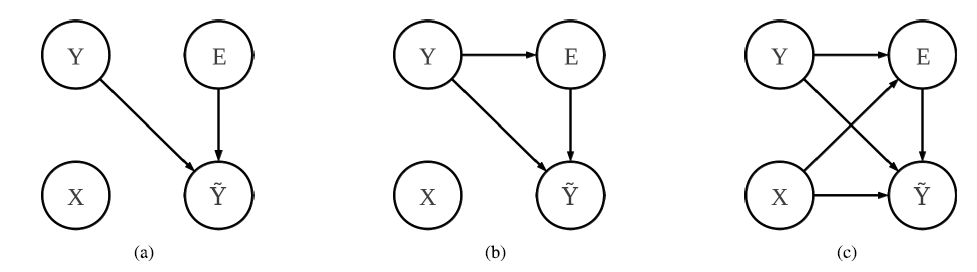
\includegraphics[clip=true, width=0.95\textwidth]{noise-taxonomy.png}
    \caption{数据标注噪音类型: (a)完全随机噪音; (b) 随机噪音; (c) 非随机噪音}\label{fig:noise-taxonomy}
\end{figure}

\begin{itemize}
    \item \textbf{完全随机噪音(NCAR)}:
        噪音$E$独立于其他随机变量,包括真实的标注$Z$。
    \item \textbf{随机噪音(NAR)}:
        噪音$E$独立于数据$X$, 但依赖真实的标注$Z$。该模型允许非对称噪音,
        即某些类别的数据更有可能出现标注噪音。随机噪音可等价地表示为一个标注矩阵或转移矩阵:
        \begin{eqnarray}
            \gamma =
            \begin{pmatrix}
                \gamma_{11} & \cdots & \gamma_{1K} \\ 
                \vdots & \ddots & \vdots \\ 
                \gamma_{K1} & \cdots & \gamma_{KK}
            \end{pmatrix}
            =
            \begin{pmatrix}
                \P(Y = 1|Z=1) & \cdots & \P(Y= K|Z=1) \\ 
                \vdots & \ddots & \vdots \\ 
                \P(Y = 1|Z=K) & \cdots & \P(Y = K|Z=K)
            \end{pmatrix}
        \end{eqnarray}
    \item \textbf{非随机噪音(NNAR)}: 上述两种噪音类型均假设标注噪音对于同一类别下的
        所有样本具有相同的影响。然而在实际场景中,上述假设不一定成立。例如,
        当样本与其他类别样本之间的距离较近时,更有可能发生错误标注。此外,
        样本分布密度较低的区域标注的可靠性也比其他区域低。在图~\ref{fig:noise-taxonomy}(c)所示的
        模型中,标注噪音$E$同时依赖于数据$X$和真实类别$Y$,错误标注更有可能
        出现在某些类别和数据空间的某些区域。非随机噪音是最有普适性
        的噪音类型。例如,分界面附近和低样本密度分布区域的标注噪音只能用非随机噪音
        来建模。
\end{itemize}

\section{相关反馈弱监督深度神经网络}
传统弱监督目标识别算法需要人工设计
一系列的特征,如全局特征(HOG),局部特征(SIFT, SURF)等。这些特征的表达能力直接
影响到图片分类的效果,不仅提高了研究人员设计特征的难度,也制约了目标识别效果的
提高。
近年来,深度卷积神经网络在图片识别上获得了巨大的成功。
2012年,Alex等人将深度卷积神经网络应用到了百万级规模的ImageNet图像识别任务上,
提出了AlexNet网络模型,通过5层的卷积神经网络,
直接从原始的图片像素中提取从浅层语义到深层语义的特征,
然后用3层的全连接神经网络作为分类器~\cite{krizhevsky2012imagenet}。
深度学习的优点在于不需要人工设计图片特征,网络通过反向传播的方式同时
学习特征提取和分类器。然而,经典的深度卷积神经网络对于数据标注的质量有很大的依赖性,
如何利用大规模弱监督社交多媒体数据训练深度卷积神经网络成为了近年来的研究热点之一。

\begin{figure}[ht]
    \center
    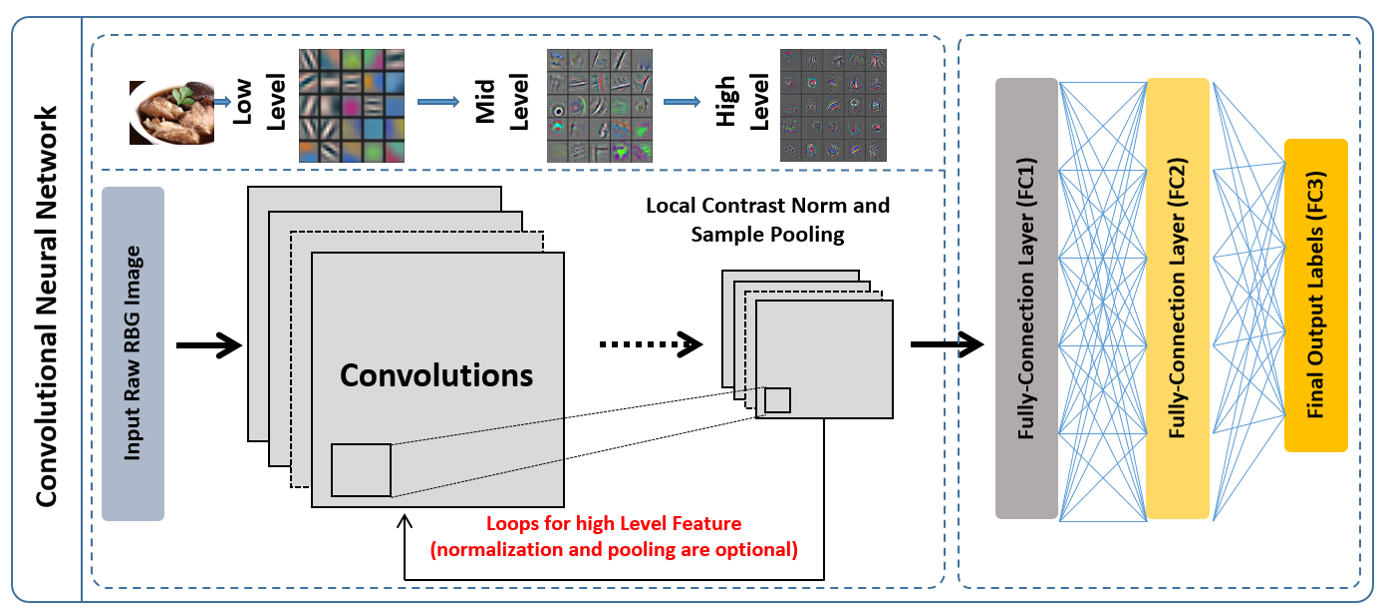
\includegraphics[clip=true, width=0.95\textwidth]{cnn.png}
    \caption{深度卷积神经网络的结构图}
    \label{fig:cnn}
\end{figure}

\subsection{经典卷积神经网络}
如图~\ref{fig:cnn}所示,经典深度卷积神经网络的前几层通常是卷积层,最后几层为全连接层,
不同的任务可能会采用不同深度的网络。最后一个全连接层的输出作为柔性最大传递函数(Softmax)
分类器的输入,得到在所有类别上的概率分布。假设训练数据为$X = [\x_1, \ldots,
\x_N]$,$\x_i$表示第i个图片, $N$是图片总数目。用$\y=[y_1, \ldots, y_N] \in
\R^{N}$表示训练数据的标注向量,$y_i \in [0,K-1]$是第i个图片的标注类别, $K$是类别数目。假设网络的层数为$M$,网络参数表示为
$W = \{W^1, \ldots, W^M\}, W^m \in \R^{d_{m-1}\times d_m}$。数据在第$m$层的特征图(Feature map)表示为
$Z^m(X) = [\z^m(\x_1), \ldots, \z^m(\x_N)]^T \in \R^{N \times d_m}$。

通常,卷积神经网络的损失函数是柔性最大传递函数的负对数似然函数和
权重衰减项(weight decay)之和:
\begin{equation}\label{eqn:cnn-loss}
    \L(W;X,\y) = -\frac{1}{N}\Big[\sum_{i=1}^N {\log p(y_i | \x_i; W)}\Big] + \frac{\beta}{2}\|W\|_F,
\end{equation}
其中,$\beta$是
权重衰减项的系数。上述损失函数相对于最后一层特征图$Z^M$以及参数$W^M$的梯度为:
\begin{eqnarray}
    Z^M &=& Z^{M-1}W^M \\
    \frac{\partial{\L(W;X,Y)}}{\partial{\z^M(\x_i)}} &=&
    -\frac{1}{N} \Big({\one_{y_i}(\z^M(\x_i)) - \p(\z^M(\x_i))}\Big) \\
    \frac{\partial{\L(W;X,Y)}}{\partial{W^M}} &=&
    (Z^{M-1})^T\frac{\partial{\L(W;X,Y)}}{\partial{\z^M(\x_i)}}\\
    &=& -\frac{1}{N}\sum_{i=1}^N {\z^{M-1}(x_i) \Big({\one_{y_i}(\z^M(\x_i))
    - \p(\z^M(\x_i))}\Big)^T}
\end{eqnarray}
其他层参数的梯度可以通过方向传播(Back
Propagation)得到~\cite{lecun1998gradient}。从上述公式可以看出,
错误的标注会导致参数梯度计算错误,并被反向传播, 使得经典的卷积神经网络
对于标注噪音十分敏感。

\subsection{相关反馈卷积神经网络}
目前已有部分工作研究弱监督深度学习, 然而现有方法大多基于特定的噪音模型,
难以处理真实的场景,或建模过于复杂,难以
训练。2014年谷歌研究团队提出的利用图片特征之间的相似性
监督网路学习,抑制错误标注影响的学习方法~\cite{reed2014training}。文章
认为,如果图片的特征之间具有相似性,那么预测的结果同样也应该比较类似,
并称之为感知连续性, 并将感知连续性应用到随机噪声假设下的网络学习中。本文
在感知连续性的基础上提出了不依赖于特定噪声类型的相关反馈卷积神经网络。

基于感知连续性,本文方法的基本假设是正确标注样本在图像空间具有相似性,
它们的特征表示在特征空间也具有相似性,而错误标注的样本则不具有这种相似性。
因此,可以利用特征之间的相关性作为反馈,
使得网络训练过程中不同数据在模型训练中发挥不同的作用。

为了表示特征之间的关系,我们将网络最后一层的特征转换为能反映
特征之间相互关系的关联特征表示(Affinity Representation)。类似于
Belkin等人提出的最近邻系统~\cite{belkin2001laplacian},我们定义如下
相似度矩阵$S\in R^{N \times N}$:
\begin{equation}\label{eqn:rf-cnn-sim}
    S_{ij} =
    \begin{cases}
        \exp\{-\frac{\|\z^M(\x_i) - \z^M(\x_j)\|^2}{\gamma^2}\} & y_i = y_j\\
        0 & \text{otherwise},
    \end{cases}
\end{equation}
$\gamma$是尺度因子。为了更好地反映相似度矩阵的局部结构,我们用一个对角矩阵$D$
对相似度矩阵进行正则化,$D_{ii} = \sum_{j=1}^N S_{ij}$。
训练数据最终的特征表示为$\Psi(X;W) = [\vpsi(\x_1), \ldots, \vpsi(\x_N)] =
D^{-1}S$,矩阵$\Psi(X;W)$的每一列包含了数据$\x_i$的特征和其他数据特征之间的关系。

假设理想情况下,不受噪音影响的模型参数为$W^*$,
则噪音鲁棒学习算法应该尽量优化$W$使其逼近$W^*$。
该优化目标可以通过最小化学习到的特征表示$\Psi(X;W)$和理想情况下的
特征表示$\Psi(X;W^*)$之间的差值$E_n$得到。$E_n$是由于噪音标注引起的特征表示的误差。
换句话说,可以认为$\Psi(X;W)$是理想特征与一个加性噪声之和:
\begin{equation}
    \Psi(X;W) = \Psi(X;W^*) + E_n
    \label{eqn:additive-noise}
\end{equation}
根据方程~\eqref{eqn:additive-noise}以及低秩理论~\cite{candes2011robust},
我们假设$\Psi(X;W^*)$是低秩矩阵:
\begin{equation}
    \text{rank}(\Psi(X;W)) > \text{rank}(\Psi(X;W^*))
\end{equation}

在社交多媒体数据上,假设类别数目足够多,
错误的标注来自于同一训练数据集上的其他类别, 并假定训练数据的特征最多有$K$个
模式,$\Psi(X;W^*)$的秩等于类别数目$K$,因此, $\Psi(X;
W^*)$可以通过如下优化方程得到:
\begin{eqnarray}
    \label{eqn:low-rank}
    \min_{\Psi(X;W^*)} \|\Psi(X;W) - \Psi(X;W^*)\|_F, \\ \nonumber
    \text{s.t.} \quad  \text{rank}(\Psi(X;W^*)) = K
\end{eqnarray}

\begin{figure}[ht]
    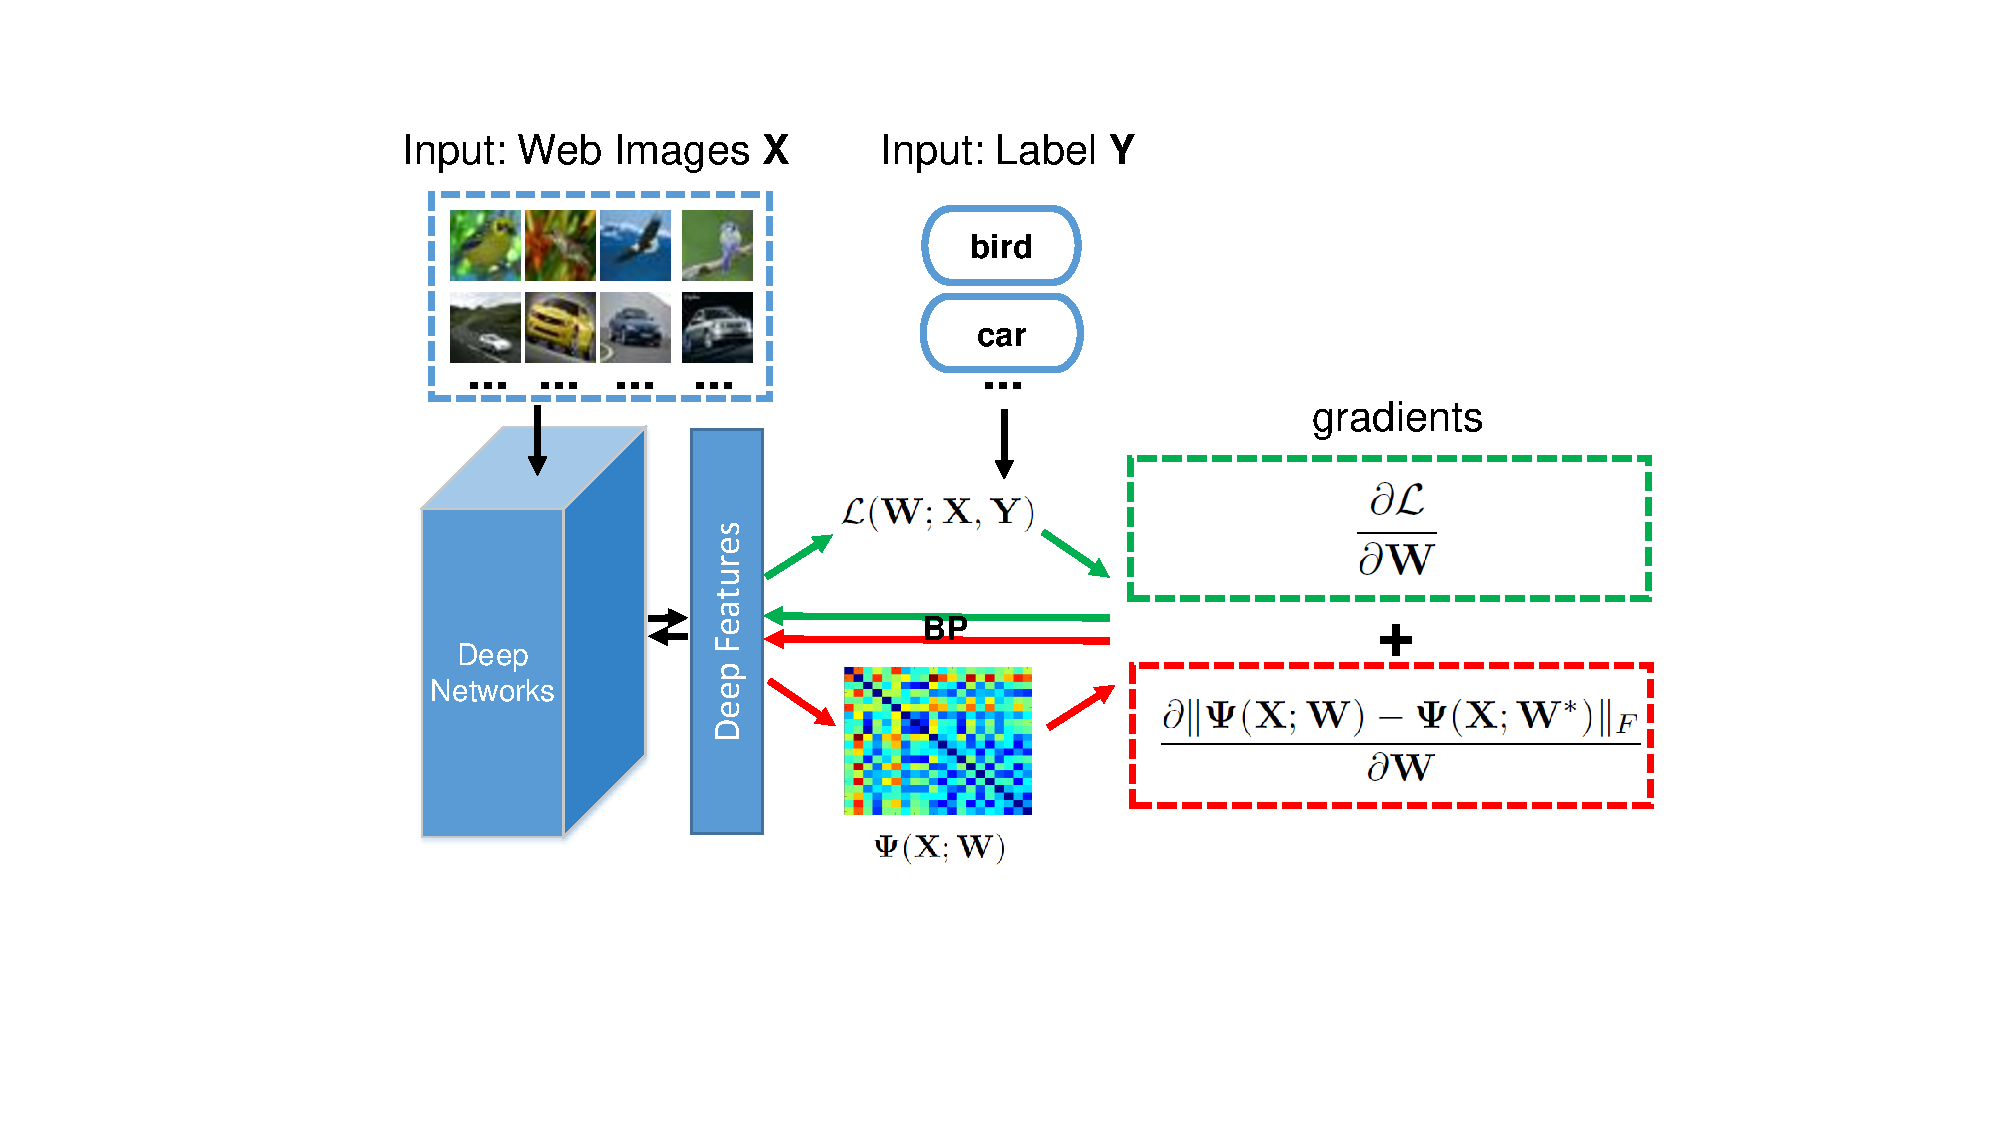
\includegraphics[clip=true, width=0.95\textwidth]{rf-cnn-frm}
    \caption{相关反馈卷积神经网络}\label{fig:rf-cnn-frm}
\end{figure}
如图~\ref{fig:rf-cnn-frm}所示,相关反馈卷积神经网络通过
特征矩阵的额重构误差,利用训练数据之间的感知连续性,
抑制训练过程中噪音的影响。
然而,由于方程~\eqref{eqn:low-rank}带来的计算量,
上述方法极大增加了优化过程的时间开销。此外,该方法优化过程分两步:
解优化方程~\eqref{eqn:low-rank}和反向传播。为了避免该方法呢的缺点,
本文进一步提出了改进的快速算法。快速算法基于下面的命题:
\begin{proposition}\label{prop:lowrank-spec}
    令$L=D-S, H^* \in R^{N\times K}$由$\Psi(X;W)$的K个最大的特征值
    对应的特征向量构成,可以得到:1)方程~\eqref{eqn:low-rank},即$\Psi(X;W)$
    的秩为$K$的最佳近似由特征向量矩阵$H^*$唯一决定;2)$H^*$也是下列优化方程的最优解:
    \begin{equation}
        \label{eqn:spec-cluster}
        \min_H \text{tr}[H^TLH] \quad \text{s.t.} \quad H^TH = I.
    \end{equation}
    由于方程~\eqref{eqn:low-rank}和方程~\eqref{eqn:spec-cluster}均在$H^*$取得
    最优值,可以认为方程~\eqref{eqn:low-rank}和方程~\eqref{eqn:spec-cluster}
    作为惩罚项是等价。
\end{proposition}
\begin{proof}
    命题~\ref{prop:lowrank-spec}可以通过如下三个定理得到。
    不失一般性,假设$\text{rank}(\Psi(X;W)) = r$。矩阵的秩为$K$
    的最小重构误差矩阵可以通过\emph{Eckart-Young-Mirsky}
    定理~\cite{eckart1936approximation}得到:
    \begin{theorem}[Eckart-Young-Mirsky]\label{thm:eym}
        对秩为$r$的矩阵$P\in \R^{m\times n}$进行奇异值分解(Singular Value
        Decomposition, SVD)得到$P=U\Sigma V^T, U^TU=I, V^TV=I$,
        如果$K < r$, 则有:
        $$%\begin{equation}
            \argmin_{
                \mbox{\scriptsize
                    $
                    \begin{array}{c}
                        \hat{P} \in \R^{m\times n} \\
                        \text{rank}(\hat{P}) = K
                    \end{array}
                    $
                }
            } \|P - \hat{P}\|_F = U\hat{\Sigma}V^T,
        $$%\end{equation}
        其中$\hat{\Sigma}$是包含$P$的前$K$个最大奇异值的对角矩阵。
    \end{theorem}

此外,如果矩阵$P$是实对称矩阵,它的奇异值和特征值之间具有如下定理所示关系:
\begin{theorem}\label{thm:evd}
    对实对称矩阵$P$特征值分解(EVD)得到$P=Q\Lambda Q^T, Q^TQ = I,
    \Lambda = \text{diag}(\lambda_1, \ldots, \lambda_N).
    \lambda_1 \geq \lambda_2 \geq \ldots \geq \lambda_N$是矩阵$P$的特征值。则有
    $$Q=U$$
\end{theorem}
因此,根据定理~\ref{thm:eym}和定理~\ref{thm:evd},实对称矩阵$\Psi(X;W)$的秩为$K$
的最小重构误差矩阵由$\Psi(X;W)$的前$K$个最大特征值对应的特征向量对应的矩阵构成。

根据Rayleigh~\cite{golub2012matrix}可以得到如下定理:
\begin{theorem}
    令$H^* = [\h_1^*, \ldots, \h_K^*] = \argmin_{H} \text{tr}[H^TLH]$,
    并且$H^TH = I$,
    则最优解$H^*$可以通过求解如下泛化特征值分解问题得到:
    $$
    L\h_i = (1-\lambda_i) D\h_i,
    $$
    其中$\{1-\lambda_i^* | i = 1,\ldots,
    K\}$是矩阵$\Psi(X;W)$的前K个最大特征值,
    $H^* = \{\h_i^* | i=1, \ldots, K\}$是对应的特征向量。
\end{theorem}
由于方程~\eqref{eqn:low-rank}和方程~\eqref{eqn:spec-cluster}均在$H^*$取得
最优值,可以认为方程~\eqref{eqn:low-rank}和方程~\eqref{eqn:spec-cluster}
作为惩罚项是等价。
\end{proof}

通过以上命题和证明可以发现,方程~\eqref{eqn:low-rank}的最优解可以通过
方程~\eqref{eqn:spec-cluster}中最小迹得到。因此,我们提出将最小迹的优化
目标引入到经典的神经网络中,最终的噪音鲁棒深度网络目标方程为:
\begin{equation}\label{eqn:rf-cnn-obj}
    \widetilde{\L} = \L(W;X,Y) + \alpha \text{tr}[H^TLH].
\end{equation}

上述优化方程仍然需要对特征矩阵进行特征值分解,本文提出了进一步的近似方法。
首先构建标注矩阵$Y = [\y_1,\ldots, \y_N]^T \in \{0,1\}^{N\times K}$, 每一列
$\y_i\in\{0,1\}^{K\times
1}$表示数据$\x_i$的标注向量,并且只有$y_i$位置为非零值。由于$Y$矩阵是在
语义空间上对数据的表述,$H$是在特征空间上的主成分表述,根据感知连续性,$H$
可以通过如下优化方程近似得到~\cite{yang2011l2,ye2008discriminative}:
\begin{equation}
    \min_{H} \|HH^T - YY^T\|_F^2.
\end{equation}
为了满足$H$矩阵的正交性,一个合理的近似解为$H = Y(Y^TY)^{-\frac{1}{2}}$。

\subsection{相关反馈分析}
为了验证上述方法有效性,我们从梯度的角度分析相关反馈对于噪声的抑制能力。
定义第$M-1$层特征之间的距离为:

TBD.

图片$\x_i$对于梯度的贡献如图~\ref{fig:rf-cnn-gradient}所示。
\begin{figure}[ht]
    \center
    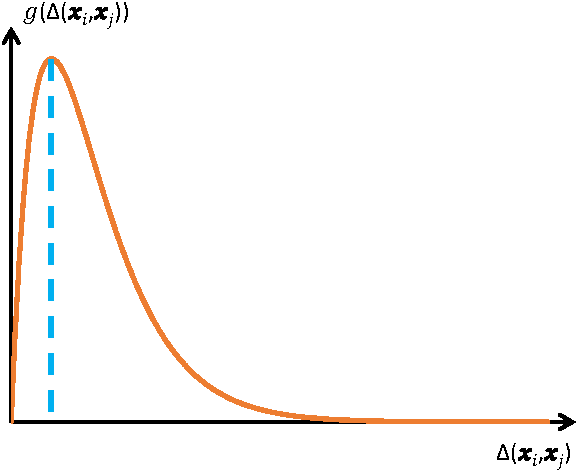
\includegraphics[clip=true, width=0.55\textwidth]{rf-cnn-gradient}
    \caption{训练数据对于梯度的贡献曲线,横坐标为数据与其他数据的距离}\label{fig:rf-cnn-gradient}
\end{figure}

\section{实验结果和评估}
本节从实验的角度验证本文提出的弱监督相关反馈卷积神经网络的有效性。
首先在标准数据集上验证该方法对于噪声标注的鲁棒性,其次,我们将该方法用于
真实的社交数据集,验证该方法在图片标注上的有效性。

\subsection{目标识别}

\textbf{实验数据}: 我们在两个公开数据集上分别验证算法对噪声的鲁棒性。
一个是CIFAR-10~\cite{krizhevsky2009learning},
包含$10$个类别$60,000$张$32\times 32$的彩色图片,其中
$50,000$用于训练,$10,000$用于测试。 为了产生不同噪声比例的训练数据,
在每个类别的训练数据上按照不同比例,随机选取图片,并将他们的类别随机替换为
数据集中的其他类别,训练数据集的总图片数目保持不变。在我们的实验设置中,
训练数据从无噪声到$90\%$的噪声均匀取$10$个噪声比例。
另一个数据集是PASCAL VOC2007~\cite{pascal-voc-2007},包含$20$个类别总共
$9,963$张图片。我们将数据集随机等分成训练数据和测试数据。

\textbf{比较基准}:本文提出的相关反馈卷积神经网络称为RFCNN,
并以下四个方法进行比较:
\begin{itemize}
    \item \textbf{CNN}: 经典的卷积神经网络。
    \item \textbf{RPCA+CNN}: 在训练卷积神经网络之前,首先用
        RPCA~\cite{candes2011robust}方法对每个训练数据进行重构,并移除重构误差较大的训练数据,
        移除的比例和噪音的比例相同。
    \item \textbf{CAE+CNN}:首先用卷积自动编码器对卷积神经网络的每一层
        进行预训练,然后微调整个网络,从而减小噪音标注的影响~\cite{luo2012hierarchical}。
    \item \textbf{NL+CNN}:用全连接层表示噪音转移概率矩阵,
        和卷积神经网络一起训练~\cite{sukhbaatar2014training}。
\end{itemize}

对于VOC2007数据集,我们还与另外两种方法进行比较:
\begin{itemize}
    \item \textbf{Best\_VOC}: 用ImageNet数据集预训练网络,
        并在VOC2007上微调~\cite{oquab2014learning}。
    \item \textbf{Web\_HOG}: 通过基于局部的模型和人工设计的特征,在网络图片上
        训练语义概念表征~\cite{divvala2014learning}。
\end{itemize}

\textbf{参数设置}:首先,我们调整公式~\eqref{eqn:cnn-loss}
中权重衰减项的系数$\beta$。对于$10\%$的噪音比例,该稀疏取$0.004$时
网路能达到最好的效果,对于$20\%$的噪音比例,取值为$0.008$,其他噪音比例下取值
为$0.04$。该参数设置对于两个数据集都能取得最好的效果。
此外,我们按照经验将公式~\eqref{eqn:rf-cnn-sim}中的$\gamma$参数设为$0.1$,使得特征相似度在合理的范围。
图~\ref{fig:rf-cnn-alpha}显示了在CIFAR-10数据集$20\%$噪音下,公式~\eqref{eqn:rf-cnn-obj}中不同$\alpha$取值
对于网络准确率的影响。我们发现,只有当$\alpha$取值过大时(比如取$10$),模型的
完全丧失了分类能力,对于其他取值,准确率都保持在相对稳定的范围,并在取值为$0.5$时
达到最优。此外,我们发现$\alpha$取$0.5$在其他噪音条件下也能取得最好的效果。因此,
以下实验$\alpha$均取$0.5$。
\begin{figure}[ht]
    \center
    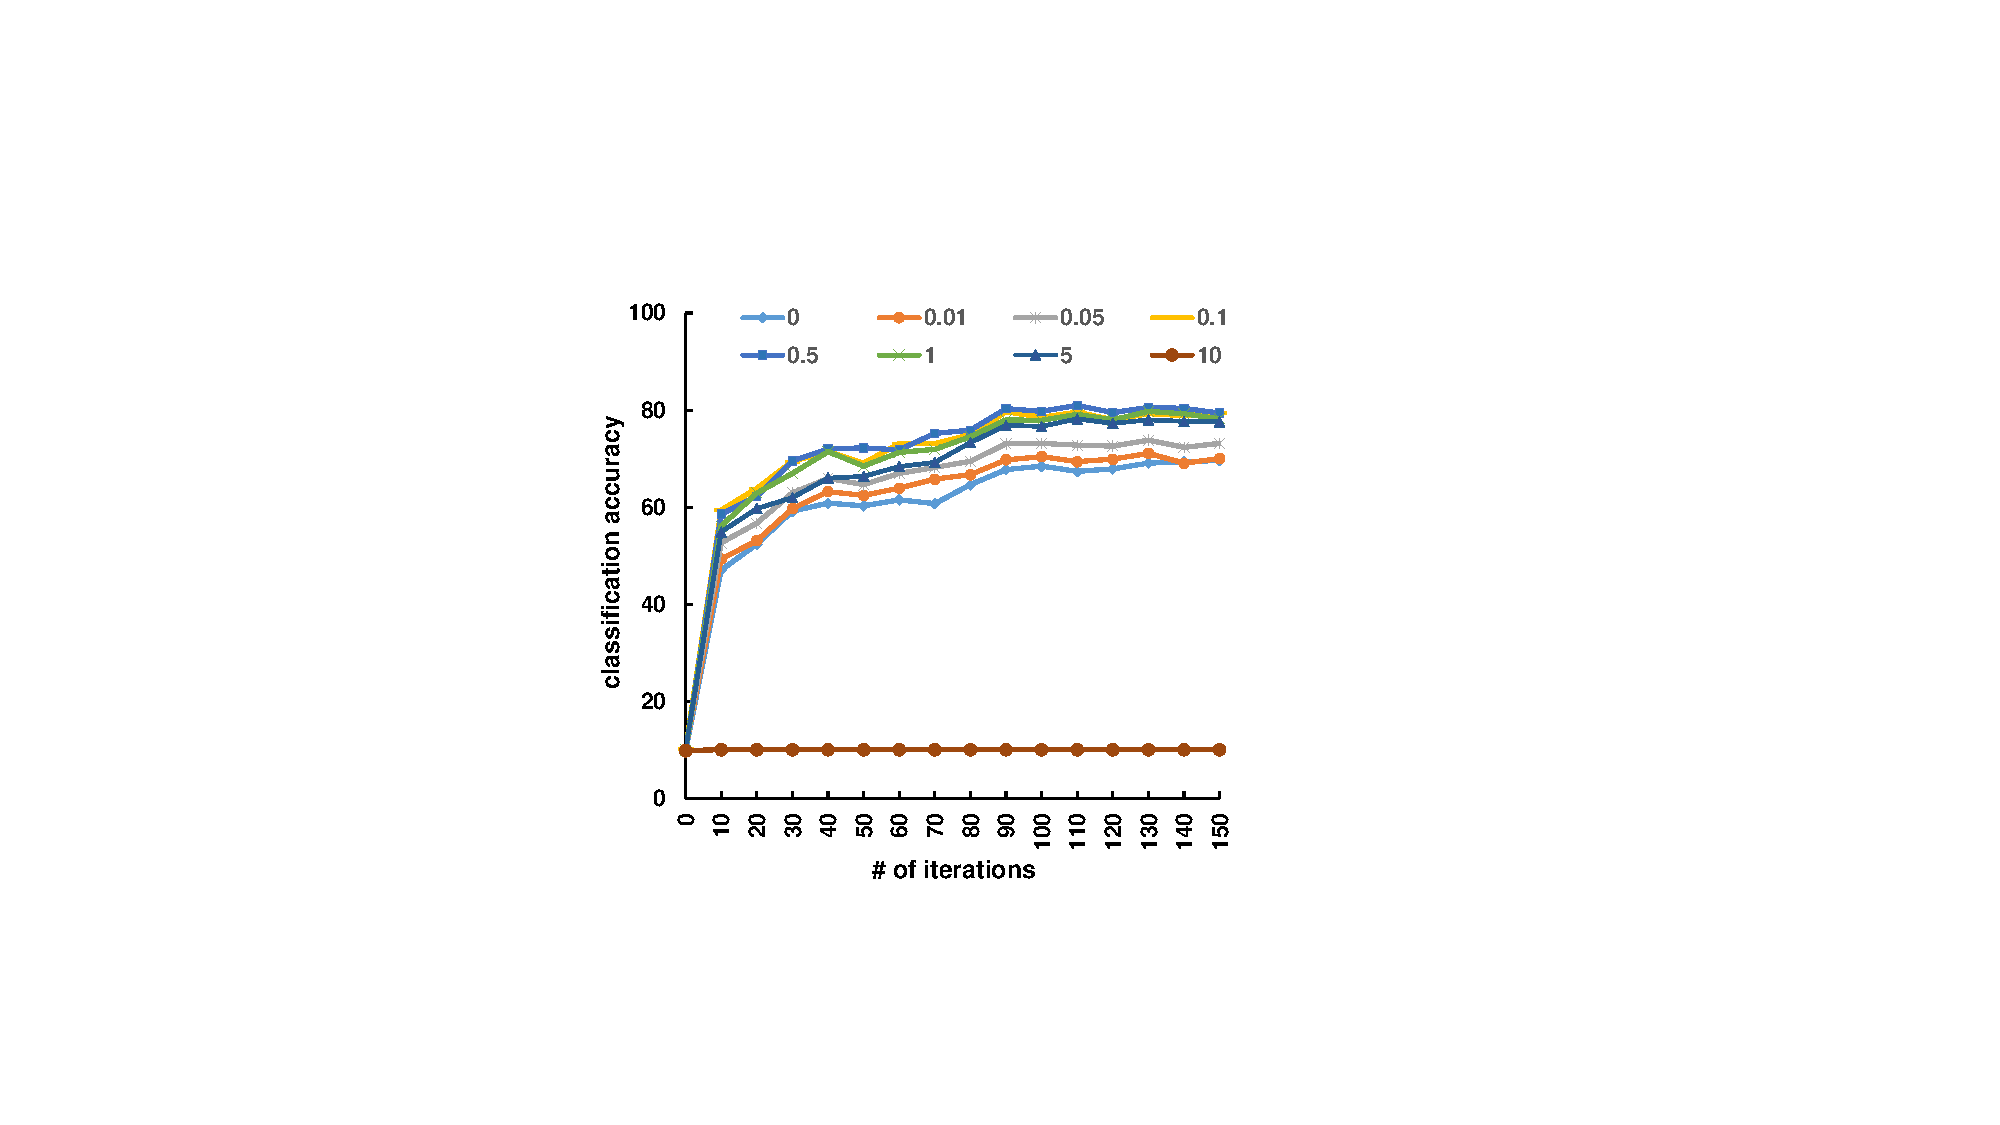
\includegraphics[clip=true, width=0.55\textwidth]{rf-cnn-alpha}
    \caption{参数$\alpha$对于卷积神经网络分类性能的影响}\label{fig:rf-cnn-alpha}
\end{figure}

\textbf{实验结果}:表格~\ref{tab:rf-cnn-cifar10}显示了在CIFAR-10数据集上不同噪音
程度下不同算法的分类准确率比较。本文提出的算法在所有条件下都达到了最好的实验结果,
甚至在无噪声数据集上,我们的算法也比经典的卷积神经网络取得了略好的准确率。我们发现,
在$30\%$噪音数据下,经典卷积神经网络的准确率下降了将近$20\%$。相比之下,本文提出的算法
值下降了$10\%$,表现出了对噪音数据很强的鲁棒性。此外,我们发现数据预处理方法RPCA+CNN在
噪音比例小于$50\%$时的准确率要好于经典的卷积神经网络,当有更多的噪音数据时,
RPCA+CNN的效果则比经典CNN要差。这个现象的原因在于当噪音数据增多时,
数据预处理移除正确数据的风险也随之增大,导致在最终的训练数据中噪音数据的比例增加。
CAE+CNN和NL+CNN算法的性能十分接近,在$30\%$噪音比例下,准确率分别下降$17.0\%$和
$15.9\%$。CAE+CNN虽然能够解决区域级的噪声(背景噪声),但对于样本集噪声(如本文中
的标注错误),它的鲁棒性则比较有限。对于NL+CNN,我们的实验证明仅仅在网路上增加一层
噪音适应层并不能噪音鲁棒性。相反,我们的方法可以抑制噪音在所有层的影响。
图~\ref{fig:rf-cnn-cifar-decline}反映了在不同噪音程度下不同方法分类准确率相对于
无噪声下降程度的比较。
\begin{figure}[ht]
    \center
    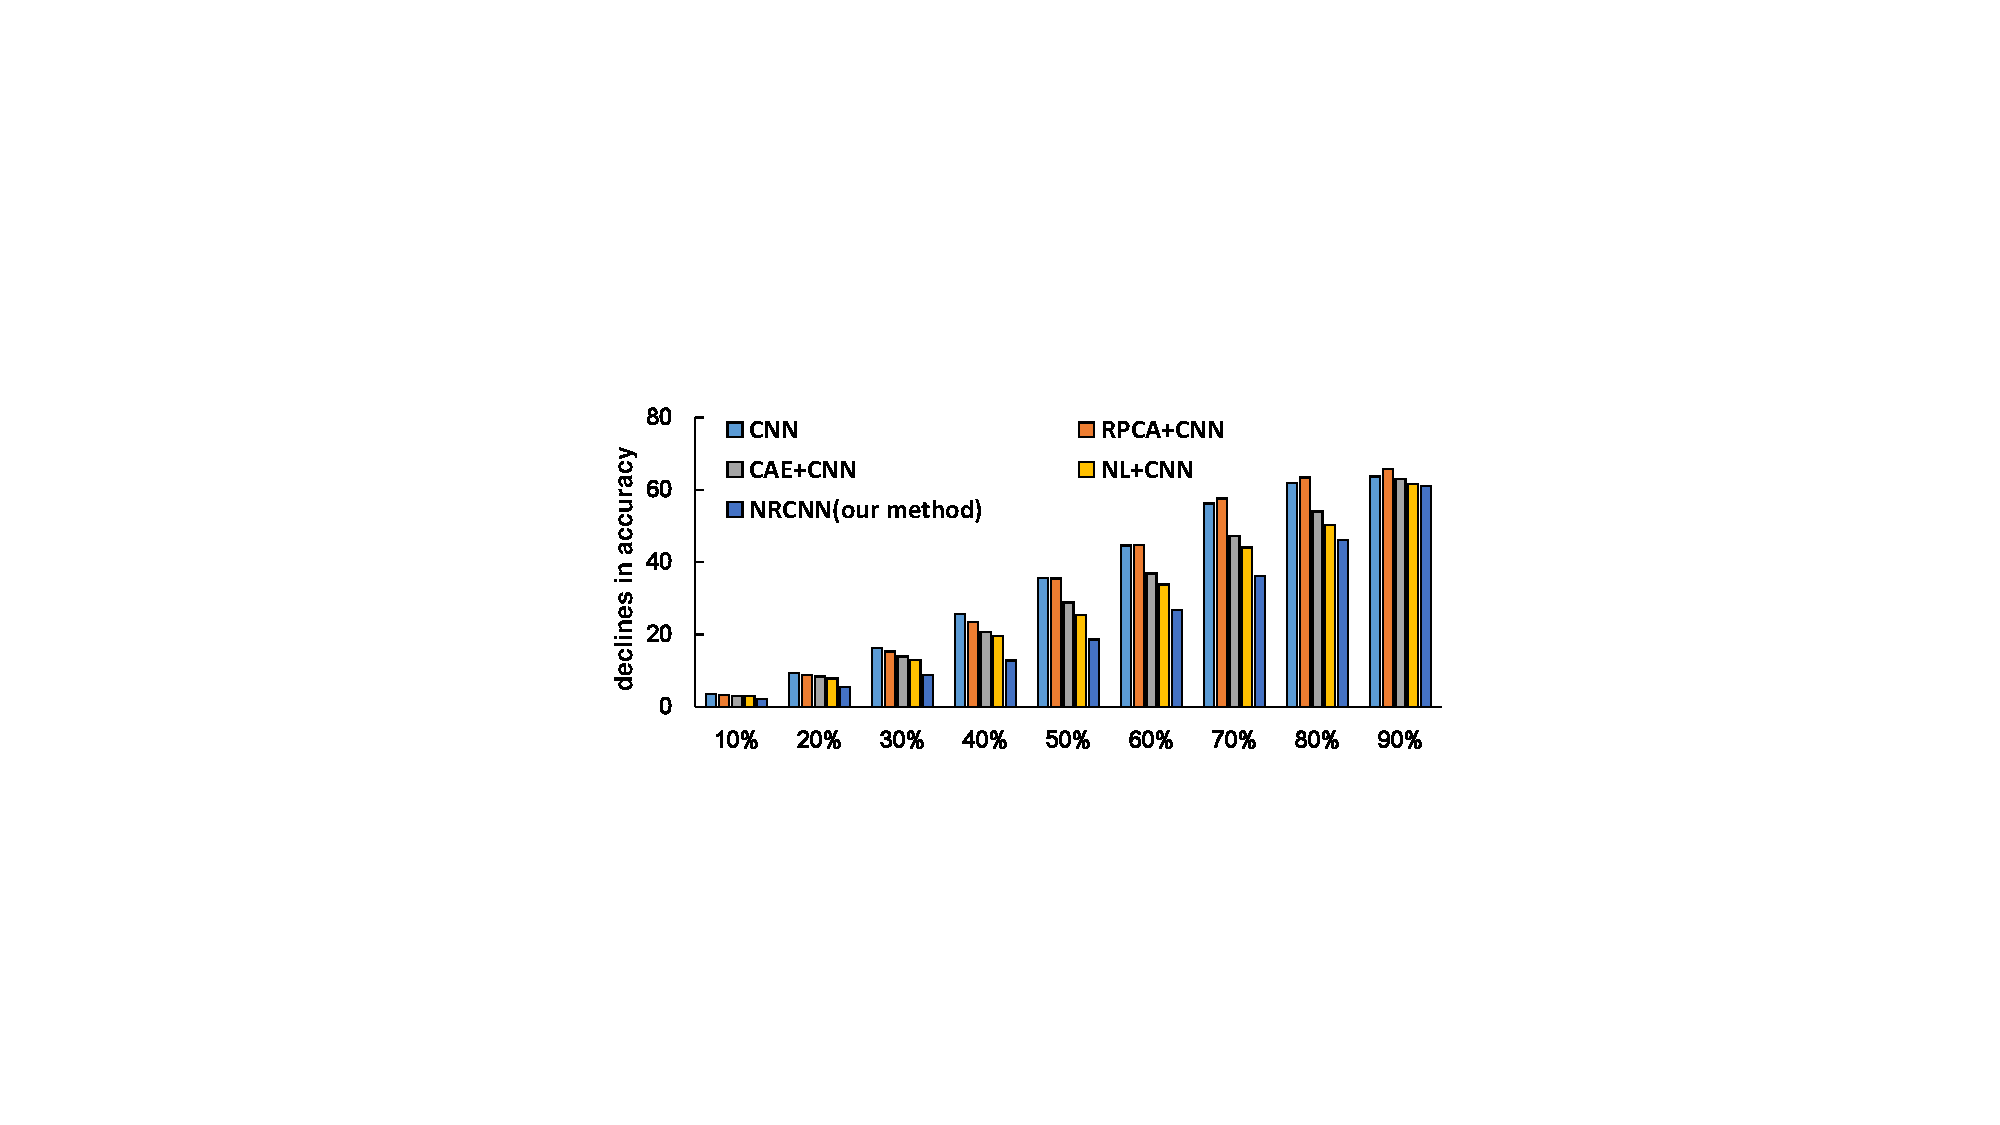
\includegraphics[clip=true, width=0.55\textwidth]{rf-cnn-cifar-decline}
    \caption{不同噪音程度下不同方法的准确率相对于无噪声的下降程度比较}
    \label{fig:rf-cnn-cifar-decline}
\end{figure}

\begin{table}[htbp]
    \centering
    \caption{不同算法在CIFAR-10数据集上不同噪音条件下的准确率比较}
    \label{tab:rf-cnn-cifar10}
    \small
    \begin{tabular}{|c|c|c|c|c|c|c|c|c|c|c|}
    \hline
    \diagbox{\scriptsize{算法}}{\scriptsize{噪声比例}} & 无噪声  & 10\% &  20\% & 30\% & 40\% & 50\% & 60\% & 70\% & 80\% & 90\% \\
    \hline
    CNN & 81.24 & 77.79 & 71.97 & 65.09 & 55.65 & 45.60 & 36.65 & 25.02 & 19.46 & 17.55 \\
    RPCA+CNN & 81.24 & 77.94 & 72.44 & 65.94 & 57.82 & 45.77 & 36.55 & 23.68 & 17.85 & 15.49\\
    CAE+CNN & 81.55 & 78.54 & 73.19 & 67.69 & 60.83 & 52.71 & 44.71 & 34.39 &
    27.54 & 18.61 \\
    NL+CNN & 81.16 & 78.28 & 73.36 & 68.26 & 61.63 & 55.83 & 47.33 & 37.12 &
    30.81 & 19.49 \\
    RFCNN & \textbf{81.60} & \textbf{79.39} & \textbf{76.21} & \textbf{72.81}
    & \textbf{68.79} & \textbf{63.01} & \textbf{54.78} & \textbf{45.48} &
    \textbf{35.43} & \textbf{20.56} \\
    \hline
\end{tabular}
\end{table}

在PASCAL VOC2007数据集上,我们使用AlexNet网络~\cite{krizhevsky2012imagenet}首先
在ImageNet数据集上预训练,然后在网络数据上微调网络参数。为了获取网络数据,
我们将数据集的每个类别作为查询词抓取搜索引擎的返回结果,并滤除重复的图片。
我们收集了两个训练数据集,第一个数据集中正负样本的数目和VOC2007中相同,
在该数据集上的实验我们记为CNN(Web)和RFCNN(Web)。第二个数据集中我们将正样本的
数目增加到VOC2007的4倍,并将该数据集上的方法记为CNN(Webx4)和RFCNN(Webx4)。
根据我们统计的结果,两个数据集上的噪音比例分别是$20\%$和$40\%$。不同方法
在VOC2007测试数据集上的平均准确率(Average Precision)如表~\ref{tab:rf-cnn-voc2007}所示。
可以发现:
\begin{itemize}
    \item
        CNN(Web)相比Web\_HOG具有十分明显的提升,证明了深度学习网络比利用人工设计的特征
        训练的分类模型具有更强的噪声鲁棒性。
    \item RFCNN(Webx4) 取得了比在大量标注好的数据集上训练的网络更好的效果。
\end{itemize}

\begin{table}[htbp]
    \centering
    \caption{不同算法在VOC2007数据集上不同噪音条件下的不同类别平均准确率比较}
    \label{tab:rf-cnn-voc2007}
    \footnotesize
    \tabcolsep=0.3mm
    \begin{tabular}{|c|c|c|c|c|c|c|c|c|c|c|c|c|c|c|c|c|c|c|c|c|c|}
    \hline
    \diagbox{\scriptsize{算法}}{\scriptsize{类别}} & plane  & bike & bird &
    boat & btl & bus & car & cat & chr & cow & tab & dog & horse & moto & pers
    & plnt & shp & sfa & train & tv & \textbf{mAP} \\
    \hline
    Best\_VOC & 88.5 & \textbf{81.5} & \textbf{87.9} & \textbf{82.0} & 47.5 &
    75.5 & \textbf{90.1} & 87.2 & 61.6 & 75.7 & \textbf{67.3} & 85.5 & 83.5 &
    80.0 & \textbf{95.6} & 60.8 & 76.8 & \textbf{58.0} & \textbf{90.4} &
    \textbf{77.9} & 77.7 \\
    Web\_HOG & 68.5 & 48.2 & 47.3 & 55.7 & 40.0 & 56.3 & 60.1 & 64.1 & 43.6 &
    59.2 & 32.9 & 46.5 & 56.2 & 62.4 & 41.3 & 29.6 & 41.4 & 35.6 & 68.9 & 35.5
    & 49.6 \\
    CNN(Web) & 84.1 & 68.8 & 77.1 & 73.0 & 63.0 & 74.2 & 74.3 & 79.2 & 61.8 &
    73.8 & 48.9 & 79.5 & 81.0 & 82.1 & 48.4 & 57.9 & 72.0 & 31.6 & 83.4 & 64.7
    & 68.9 \\
    CNN(Webx4) & 85.4 & 69.4 & 77.1 & 74.5 & 63.7 & 74.7 & 75.0 & 81.6 & 62.3 &
    75.7 & 53.3 & 80.2 & 83.8 & 84.6 & 50.7 & 58.9 & 75.9 & 41.0 & 84.5 & 69.1
    & 71.1 \\
    RFCNN(Web) & 85.8 & 69.7 & 77.4 & 75.1 & 63.8 & 75.8 & 75.6 & 82.7 & 62.7 &
    76.9 & 53.5 & 80.6 & 84.7 & 84.9 & 49.2 & 59.1 & 76.0 & 50.8 & 84.8 & 69.2
    & 71.9 \\
    RFCNN(Webx4) & \textbf{91.3} & 75.2 & 83.3 & 81.5 & \textbf{70.2} &
    \textbf{81.3} & 80.6 & \textbf{88.3} & \textbf{67.0} & \textbf{82.5} & 60.0
    & \textbf{86.3} & \textbf{90.0} & \textbf{90.3} & 75.8 & \textbf{64.8} &
    \textbf{81.0} & 57.8 & 89.9 & 74.9 & \textbf{78.6} \\ 
    \hline
\end{tabular}
\end{table}

\section{小结}



